\documentclass[a4paper]{article}

%use the english line for english reports
%usepackage[english]{babel}
\usepackage[portuguese]{babel}
\usepackage[utf8]{inputenc}
\usepackage{indentfirst}
\usepackage{graphicx}
\usepackage{verbatim}
\usepackage{listings}
\usepackage{float}


\begin{document}

\setlength{\textwidth}{16cm}
\setlength{\textheight}{22cm}

\title{\Huge\textbf{Xadrersi}\linebreak\linebreak\linebreak
\Large\textbf{Relatório Final}\linebreak\linebreak
\linebreak\linebreak

\includegraphics[scale=0.1]{feup-logo.png}\linebreak\linebreak
\linebreak\linebreak
\Large{Mestrado Integrado em Engenharia Informática e Computação} \linebreak\linebreak
\Large{Programação em Lógica}\linebreak
}

\author{\textbf{Grupo Xadrersi\_1:}\\ António Cunha Seco Fernandes de Almeida - up201505836 \\ João Paulo Madureira Damas - up201504088 \\\linebreak\linebreak \\
 \\ Faculdade de Engenharia da Universidade do Porto \\ Rua Roberto Frias, s\/n, 4200-465 Porto, Portugal \linebreak\linebreak\linebreak
\linebreak\linebreak\vspace{1cm}}
\date{12 de novembro de 2017}
\maketitle
\thispagestyle{empty}

%************************************************************************************************
%************************************************************************************************

\newpage

\section*{Resumo}
Resumo sucinto do trabalho com 150 a 250 palavras (problema abordado, objetivo, como foi o problema resolvido/abordado, principais resultados e conclusões).

\newpage

\tableofcontents

%************************************************************************************************
%************************************************************************************************

%*************************************************************************************************
%************************************************************************************************

\newpage

%%%%%%%%%%%%%%%%%%%%%%%%%%
\section{Introdução}

Descrever os objetivos e motivação do trabalho. Descrever num parágrafo breve a estrutura do relatório.


%%%%%%%%%%%%%%%%%%%%%%%%%%
\section{O Jogo Xadrersi}

\textbf{Origens}\linebreak

Xadrersi é um jogo de tabuleiro para duas pessoas criado por Andi Lewicki, em 2003. Como o nome sugere, surge de uma combinação entre os conhecidos jogos de tabuleiro Xadrez e Reversi.\newline

\textbf{Regras}\newline

O jogo é disputado num tradicional tabuleiro 8x8, inicialmente vazio. A seu dispor, cada jogador possui as peças de que disporia se estivesse numa partida de Xadrez, exceto peões.
Por outras palavras, cada jogador possui um rei, uma rainha, dois cavalos, dois bispos e duas torres.\newline

Os jogadores vão colocando as suas peças no tabuleiro, uma a uma, alternadamente, até todas as peças estarem em jogo.
Após colocada, uma peça não pode ser movida nem retirada (capturada).
No entanto, ataca outras posições do tabuleiro segundo as regras de Xadrez (o rei ataca as posições adjacentes, o bispo diagonalmente, o cavalo em 'L', etc).
Não se aplicam regras de cheque nem afastamento obrigatório entre reis, logo um rei pode ser colocado numa posição onde ficaria em cheque e os reis podem ficar em posições adjacentes. \textit{(Manter ou remover consoante regra estiver implementada?) Os bispos devem ficar em posições de cores opostas, como no Xadrez.}\newline

De uma maneira geral, cada jogada é válida se e só se a peça colocada estiver a ser atacada por pelo menos uma peça adversária. A primeira exceção a esta regra é a primeira jogada, em que não há peças no tabuleiro. O jogador com as peças brancas começa e a primeira peça jogada é obrigatoriamente o rei, podendo ser colocado em qualquer posição.
As figuras \ref{fig:fig1}, \ref{fig:fig2} e \ref{fig:fig3} ilustram uma sequência de jogadas válidas (com as hipóteses em cada turno destacadas) a partir da posição inicial.


\begin{tiny}
\begin{figure}[H]
\minipage{0.2\textwidth}
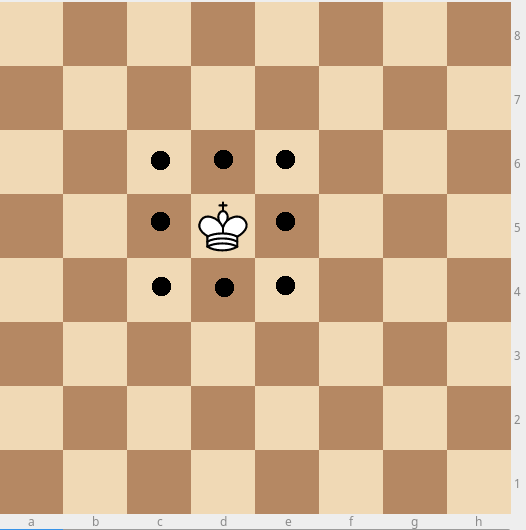
\includegraphics[scale=0.2]{board1.png}
\caption{\textit{Após a primeira jogada, uma peça preta tem de ser colocada adjacentemente ao rei branco de modo a poder ser atacada por este, constituindo uma jogada válida}}
\label{fig:fig1}
\endminipage\hfill
\minipage{0.2\textwidth}
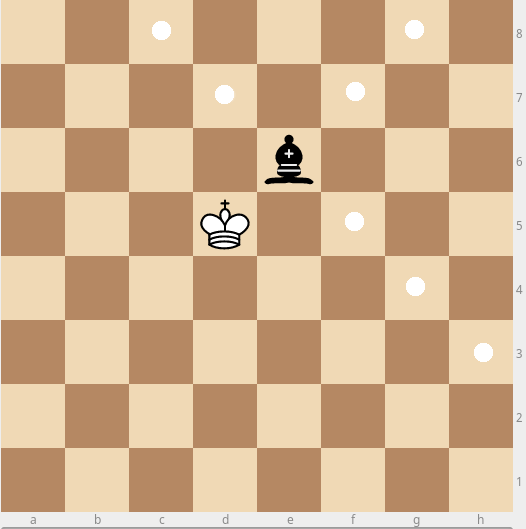
\includegraphics[scale=0.2]{board2.png}
\caption{\textit{Agora, tendo o jogador de peças pretas jogado um bispo, o jogador de peças brancas deve colocar uma peça que intersete o mesmo segundo uma das suas diagonais livres}}
\label{fig:fig2}
\endminipage\hfill
\minipage{0.2\textwidth}
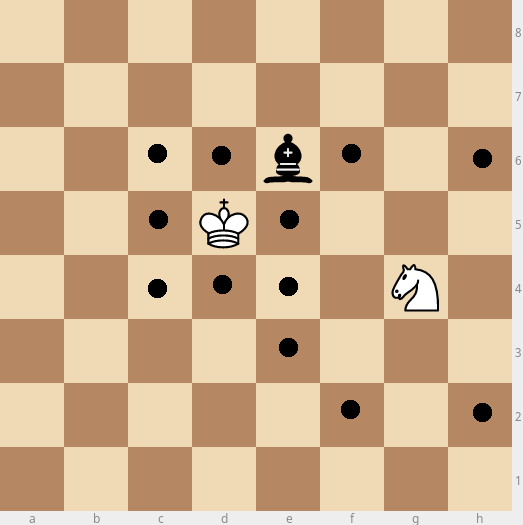
\includegraphics[scale=0.2]{board3.png}
\caption{\textit{Neste caso, tendo já mais do que uma peça branca em jogo, o jogador de peças pretas apenas precisa de se certificar que a peça que colocar é atacada por pelo menos uma peça branca}}
\label{fig:fig3}
\endminipage
\end{figure}
\end{tiny}


Existe ainda outro caso excecional. Caso seja impossível colocar uma peça de tal modo que seja atacada por uma peça adversária, o jogador pode colocar a peça em qualquer posição livre no tabuleiro. Na figura \ref{fig:fig4} demonstra-se esta situação através de um caso simples.

\begin{tiny}
\begin{figure}[H]
\begin{center}
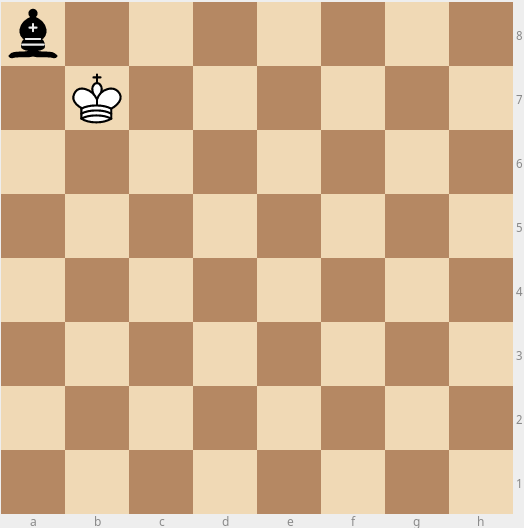
\includegraphics[scale=0.25]{board4.png}
\caption{\textit{Após a jogada inicial do rei, o bispo foi colocado em A8, adjacente ao rei e por isso válido. No entanto, a sua única diagonal está bloqueada e por isso nenhuma posição livre é atacada pelo mesmo. Nesta situação, aplica-se a exceção e a próxima peça branca pode ser colocada em qualquer posição livre.}}
\label{fig:fig4}
\end{center}
\end{figure}
\end{tiny}


Para além da obrigatoriedade do rei branco ser a primeira peça jogada, existem ainda duas regras adicionais a assinalar para tentar garantir o equilíbrio do jogo:
\begin{itemize}
    \item O rei preto é sempre a última peça a ser colocada no tabuleiro
    \item Quando um jogador coloca em jogo a sua rainha, o outro é obrigado, no turno seguinte, a colocar também a sua rainha em jogo
\end{itemize}

\textbf{Objetivo}\newline

O objetivo é conseguir o maior número de pontos quando o jogo terminar, ou seja, quando todas as peças forem colocadas no tabuleiro.
O número de pontos de um jogador corresponde ao número total de casas que as suas peças atacam.
Caso várias peças ataquem a mesma casa, esta é contabilizada uma vez por cada peça que a ataca.
Existe, por isso, a possibilidade de empate.

%%%%%%%%%%%%%%%%%%%%%%%%%%
\section{Lógica do Jogo}

\subsection{Representação do Estado do Jogo}
\textit{TODO: Em vez disto, falar da 'classe' Game e deixar apenas do que está atualmente os tabuleiros de estado de jogo (com uma frase de introdução a dizer que as peças são guardadas pelos carateres/códigos ASCII)?}
De forma a sistematizar uma relação entre a representação interna das pecas de jogo com a visualização das mesmas na consola, foi definida uma convenção. Os caracteres internamente baseiam-se na nomenclatura em inglês das peças de Xadrez, distinguindo-se as cores das mesmas através da utilização de maiúsculas ou minúsculas. Na prática, são guardados os códigos ASCII destes carateres.
Para representar no ecrã são utilizados os códigos Unicode existentes para as peças de Xadrez, como observável na subsecção seguinte.

\begin{small}
\minipage{0.3\textwidth}

\large Peças Brancas
\begin{center}
  \begin{tabular}{ l | c | r }
    Rei & 'K' & 75 \\ \hline
    Rainha & 'Q' & 81 \\ \hline
    Bispo & 'B' & 66\\ \hline
    Cavalo & 'N' & 78\\ \hline
    Torre & 'R' & 82\\
  \end{tabular}
\end{center}

\endminipage\hfill
\minipage{0.3\textwidth}

\large Peças Pretas
\begin{center}
  \begin{tabular}{ l | c | r }
    Rei & 'k' & 107\\ \hline
    Rainha & 'q' & 113\\ \hline
    Bispo & 'b' & 98\\ \hline
    Cavalo & 'n' & 110\\ \hline
    Torre & 'r' & 114\\
  \end{tabular}
\end{center}

\endminipage
\end{small} \newline\newline

Por último, uma casa vazia é internalmente representada como 0 e visualizada na consola como um espaço vazio. \newline

\large Estado Inicial de Jogo
\begin{small}
\begin{center}
\begin{tabular}{c}
\begin{lstlisting}
[[  0,   0,   0,   0,   0,   0,   0,   0],
[  0,   0,   0,   0,   0,   0,   0,   0],
[  0,   0,   0,   0,   0,   0,   0,   0],
[  0,   0,   0,   0,   0,   0,   0,   0],
[  0,   0,   0,   0,   0,   0,   0,   0],
[  0,   0,   0,   0,   0,   0,   0,   0],
[  0,   0,   0,   0,  0,    0,   0,   0],
[  0,   0,   0,   0,  0,    0,   0,   0]]
\end{lstlisting}
\end{tabular}
\end{center}
\end{small}

\large Possível Estado Intermédio
\begin{small}
\begin{center}
\begin{tabular}{c}
\begin{lstlisting}
[[  0,   0,   0,   0,   0,   0,   0,   0],
[  0,   0,   0,   0,   0,   0,   0,   0],
[  0,   0,   0,   0, 114,   0,   0,   0],
[  0,   0,   0,   0,   0,   0,  78,   0],
[  0,   0,   0,  75,   0,   0,   0,   0],
[  0,   0,   0,   0,  98,   0,   0,   0],
[  0,   0,   0,   0,  0,    0,   0,   0],
[  0,   0,   0,   0,  0,    0,   0,   0]]
\end{lstlisting}
\end{tabular}
\end{center}
\end{small}

\large Possível Estado Final
\begin{small}
\begin{center}
\begin{tabular}{c}
\begin{lstlisting}
[[ 10,   0,   0,   0,   0,   0,   0,   0],
[  0,   0,   0, 110,   0,   0, 107,  82],
[  0,  78,   0,  66, 114,  81,   0,   0],
[  0,   0,   0,   0,   0,  98,  78,   0],
[  0,   0, 113,  75,  66,   0,   0,   0],
[  0,   0,   0,   0,  98,   0,   0,   0],
[  0,   0,   0,   0,   0,   0, 110,   0],
[  0,   0,  82,   0,   0,   0,   0,   0]]
\end{lstlisting}
\end{tabular}
\end{center}
\end{small}

\subsection{Visualização do Tabuleiro}
Em modo de texto, são utilizados os predicados seguintes para produzir uma representação do tabuleiro de jogo. Bocados de código estão omitidos com reticências - '(...)' - por se tratarem de repetições de carateres ou padrões de caracteres.\linebreak

\begin{small}
\begin{lstlisting}[language=Prolog]
getPieceDisplay(0, 32). % space

%white pieces
getPieceDisplay('K', 9812). % king
getPieceDisplay('Q', 9813). % queen
getPieceDisplay('R', 9814). % rook
getPieceDisplay('B', 9815). % bishop
getPieceDisplay('N', 9816). % knight

%black pieces
getPieceDisplay('k', 9818). % king
getPieceDisplay('q', 9819). % queen
getPieceDisplay('r', 9820). % rook
getPieceDisplay('b', 9821). % bishop
getPieceDisplay('n', 9822). % knight

displayBoard( Board ) :-
	displayBoardHeader,
	N is 8,
	displayBoardTail(Board, N),
	displayBottom.

displayBoardTail([], 0).

displayBoardTail( [ Row | T ], N ):-
	write('---------------------------------'), nl,
	displayRow(Row, N), nl,
	N1 is N-1,
	displayBoardTail(T, N1).

displayRow([], N):-
	write('| '), displayNumber(N).

displayRow( [ CurrentPiece | T ] , N ):-
	write('| '),
	getPieceDisplay(CurrentPiece, PieceDisplay),
	put_code(PieceDisplay),
	write(' '),
	displayRow(T, N).

displayBoardHeader:-
	nl,
	write('  a   b   c   d   e   f   g   h '),
	nl.

displayBottom:-
	write('---------------------------------'), nl.

displayNumber(N) :- write(N), !.
\end{lstlisting}
\end{small}

Os exemplos de estados de jogo apresentados acima, vistos na consola, podem observar-se nas figuras \ref{fig:fig5}, \ref{fig:fig6} e \ref{fig:fig7}:

\begin{tiny}
\begin{figure}[H]
\minipage{0.2\textwidth}
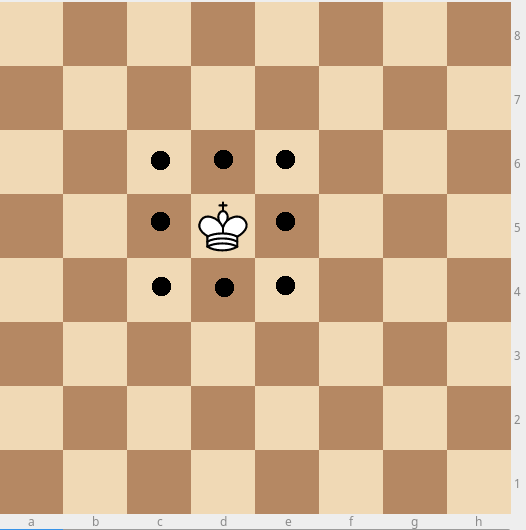
\includegraphics[scale=0.2]{board1.png}
\caption{\textit{Representação textual do estado de jogo inicial.}}
\label{fig:fig5}
\endminipage\hfill
\minipage{0.2\textwidth}
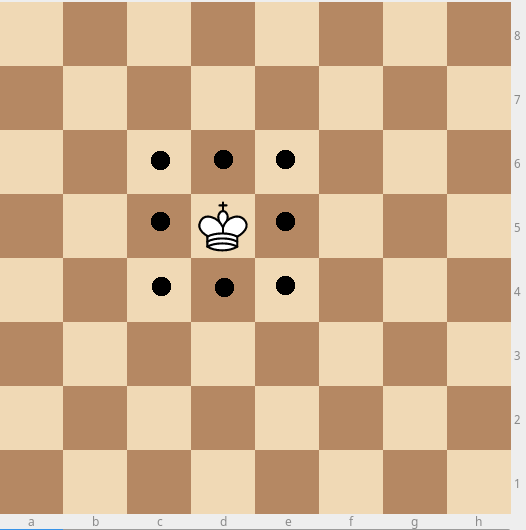
\includegraphics[scale=0.2]{board1.png}
\caption{\textit{Representação textual do estado de jogo intermédio.}}
\label{fig:fig6}
\endminipage\hfill
\minipage{0.2\textwidth}
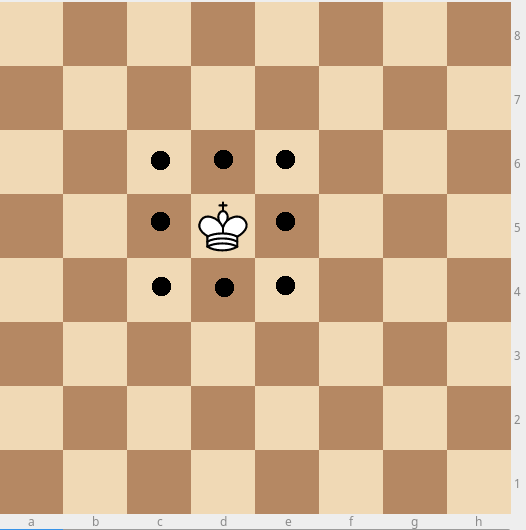
\includegraphics[scale=0.2]{board1.png}
\caption{\textit{Representação textual do estado de jogo final.}}
\label{fig:fig7}
\endminipage
\end{figure}
\end{tiny}

\subsection{Lista de Jogadas Válidas}
\textit{TODO: Falar das funções que de facto existem para isto mas só são usadas para AI, para jogadores humanos a jogada é simplesmente testada com o tabuleiro auxiliar de posições atacadas que é atualizado a cada jogada}

\subsection{Execução de Jogadas}
Após ter a informação relativa à próxima jogada, esta é primeiramente verificada quanto à sua validez e, em caso positivo, é executada.
Para validar a jogada é executada a função validMove que, consoante o tipo de jogada testa a validade de uma forma diferente.

Após a jogada ser validada, a peça é colocada no tabuleiro através da função makeMove.
Note-se que alguns excertos de código abaixo foram substituídos por comentários de forma a simplificar, minimizar o tamanho ocupado e destacar as partes mais importantes.

\begin{small}
\begin{lstlisting}[language=Prolog]
% % % % % % % % % % % % % % %
% % % % MOVE VALIDATION % % %
% % % % % % % % % % % % % % %
% first move, white king needs to be played
validateMove( Game, Player, Piece, X, Y ):-
	% check if it's the game's first move
	!,
	getBoard( Game, Board ),
	isEmpty( Board, X, Y ),
	isKing( Piece, Player ).

% final move, black king needs to be played
validateMove( Game, Player, Piece, X, Y ):-
	% check if it's the game's last move
	!,
	\+piecePlayed( Game, Player, Piece ),
	getBoard( Game, Board ),
	isEmpty( Board, X, Y),
	isKing( Piece, Player ),
	asserta( gameOver(currentGame)).

% move where player is forced to use queen
validateMove( Game, Player, Piece, X, Y ):-
	needsToPlayQueen( Game, Player ),
	!,
	isQueen( Piece, Player ),
	getBoard( Game, Board ),
	isEmpty( Board, X, Y ),
    %below is the check to see if desired cell is attacked by other player's pieces
    %code block hidden in other predicates for size purposes
	otherPlayer( Player, Other ),
	getAttackedBoard( Game, Other, AttackedBoard ),
	getPieceAt( AttackedBoard, X, Y, Value ),
	Value \== 0.

% move where first player uses queen
validateMove( Game, Player, Piece, X, Y ):-
	\+piecePlayed( Game, Player, Piece ),
	isQueen( Piece, Player ),
	getBoard( Game, Board ),
	isEmpty( Board, X, Y ),
	%check if desired cell is attacked by other player's pieces

% regular move
validateMove( Game, Player, Piece, X, Y ):-
	\+isQueen( Piece, Player ),
	\+isKing( Piece, Player ),
	\+piecePlayedTwice( Game, Player, Piece ),
	getBoard( Game, Board ),
	isEmpty( Board, X, Y ),
	%check if desired cell is attacked by other player's pieces

% special case (other player's pieces aren't attacking any cell)
validateMove( Game, Player, Piece, X, Y ):-
	\+isQueen( Piece, Player ),
	\+isKing( Piece, Player ),
	\+piecePlayedTwice( Game, Player, Piece ),
	getBoard( Game, Board ),
	otherPlayer( Player, Other ),
	getAttackedBoard( Game, Other, AttackedBoard ),
    %check that no free cells are attacked at the moment
	noFreeCells( Board , AttackedBoard ),
	isEmpty( Board, X, Y ).

noFreeCells( Board, AttackedBoard ):-
	noFreeCellsLine( Board, AttackedBoard).

% checks if line each is either occupied and attacked OR not attacked
noFreeCellsLine( [ CurrLine | RemLines ], [ CurrAttLine | RemAttLines ]):-
	noFreeCellsPiece( CurrLine, CurrAttLine ),
	noFreeCellsLine( RemLines, RemAttLines ).

noFreeCellsLine( [], [] ).

% checks if cell isn't playable because it isn't being attacked
noFreeCellsPiece( [ Cell | RemCells ], [ AttCell | RemAttCells ]):-
	AttCell == 0,
	noFreeCellsPiece( RemCells, RemAttCells ).

% checks if cell isn't playable due to being attacked but also occupied
noFreeCellsPiece( [ Cell | RemCells ], [ AttCell | RemAttCells ]):-
	AttCell \== 0,
	Cell \== 0,
	noFreeCellsPiece(RemCells, RemAttCells ).

noFreeCellsPiece( [], [] ).

makeMove( Board, Piece, X, Y, NewBoard ):-
	isWithinLimits(X),
	isWithinLimits(Y),
	N is 0,
	makeMoveAux( Board, N, Piece, X, Y, [], NewBoard ).

% % % % % % % % % % % % % % %
% % % % MOVE EXECUTION % % % %
% % % % % % % % % % % % % % %
% case where X or Y is off limits
makeMove( Board, Piece, X, Y, NewBoard ):-
	NewBoard = Board.

% base case - need to reverse list
makeMoveAux([], _, _, _, _, InvertedBoard, FinalBoard):-
	reverse(InvertedBoard, FinalBoard).

% case where N == Y
makeMoveAux([CurrentLine|RestOfBoard],Y,Piece,X,Y,TempBoard,FinalBoard):-
	N1 is Y+1,
	replace( CurrentLine, X, Piece, NewLine ),
	makeMoveAux(RestOfBoard,N1,Piece,X,Y,[NewLine|TempBoard],FinalBoard).

makeMoveAux([CurrentLine|RestOfBoard],N,Piece,X,Y,TempBoard,FinalBoard):-
	N1 is N+1,
	makeMoveAux(RestOfBoard,N1,Piece,X,Y,[CurrentLine|TempBoard],FinalBoard).
\end{lstlisting}
\end{small}

\subsection{Avaliação do Tabuleiro}
A avaliação de um determinado estado de jogo depende diretamente do tabuleiro auxiliar de posições atacadas pelo jogador.
Visto que a pontuação resulta da soma do número de posições atacadas, a avaliação é feita pelo método de cálculo da pontuação final.
Assim, uma jogada que naquele momento produza um maior número total de casas atacadas é considerada a melhor jogada.
A função de avaliação recebe o tabuleiro auxiliar de peças atacadas gerado a partir do tabuleiro de jogo naquele momento e soma os valores em casa posição (que representam o número de peças que atacam aquela posição).

\begin{small}
\begin{lstlisting}[language=Prolog]
evaluateBoard( Board, Score ):-
	evaluateBoardAux( Board, 0, Score ).

evaluateBoardAux( [ CurrentLine | RestOfBoard ], CurrentScore, Score ):-
	evaluateBoardLine( CurrentLine, 0, LineScore ),
	Temp is LineScore+CurrentScore,
	evaluateBoardAux( RestOfBoard, Temp, Score ).

evaluateBoardAux( [], Score, Score ).

evaluateBoardLine( [ N | RestOfLine ], CurrentScore, Score):-
	Temp is CurrentScore + N,
	evaluateBoardLine( RestOfLine, Temp, Score ).

evaluateBoardLine( [ 0 | RestOfLine ], CurrentScore, Score ):-
	evaluateBoardLine( RestOfLine, CurrentScore, Score ).

evaluateBoardLine( [], Score, Score ).
\end{lstlisting}
\end{small}

\subsection{Final do Jogo}
A primeira definição do predicado de ciclo de jogo playGame testa o facto gameOver com o jogo atual, facto que é só adicionado após a última peça (rei preto) tiver sido jogada, através da chamada asserta.
Caso o jogo tenha de facto terminado, a pontuação de cada jogador é calculada através da função de avaliação e é imprimida a cor vencedora.

\begin{small}
moveValidation.pl:
\begin{lstlisting}[language=Prolog]
% final move, black king needs to be played
validateMove( Game, Player, Piece, X, Y ):-
    %check move validity (code hidden)
    asserta( gameOver(currentGame)).
\end{lstlisting}
\end{small}

\begin{small}
game.pl:
\begin{lstlisting}[language=Prolog]
playGame( Game ):-
    gameOver( currentGame ),
    getAttackedBoard( Game, white, AttackedBoardWhite ),
    getAttackedBoard( Game, black, AttackedBoardBlack ),

    evaluateBoard( AttackedBoardWhite, WhiteScore ),
    evaluateBoard( AttackedBoardBlack, BlackScore ),

    displayWinner( WhiteScore, BlackScore ).

    displayWinner( White, Black ):-
    	White > Black,
    	write('!!!!!!!!!!!!'),
    	write('!White Wins!'),
    	write('!!!!!!!!!!!!').

    displayWinner( White, Black ):-
    	emoji(trophy),
        (...)
    	emoji(trophy), nl,
    	emoji(trophy),
    	write(' Black Wins '),
    	emoji(trophy), nl,
    	(...)
    	emoji(trophy).
\end{lstlisting}
\end{small}

\subsection{Jogada do Computador} Escolha da jogada a efetuar pelo computador, dependendo do nível de dificuldade. Por exemplo: \textit{choose\_move(+Level, +Board, -Move)}.


%%%%%%%%%%%%%%%%%%%%%%%%%%
\section{Interface com o Utilizador}

Descrever o módulo de interface com o utilizador em modo de texto.


%%%%%%%%%%%%%%%%%%%%%%%%%%
\section{Conclusões}
Que conclui deste projecto? Como poderia melhorar o trabalho desenvolvido?


\clearpage
\addcontentsline{toc}{section}{Bibliografia}
\renewcommand\refname{Bibliografia}
\bibliographystyle{plain}
\bibliography{myrefs}

\newpage
\appendix
\section{Nome do Anexo}
Código Prolog implementado devidamente comentado e outros elementos úteis que não sejam essenciais ao relatório.

\end{document}
